\section{Microcomputer Organization}
\subsection{Base Microcomputer Structure}
\begin{minipage}{0.7\linewidth}
	\begin{itemize}
		\item Central Processing Unit (CPU)
		\subitem Fetch, Decod and Executes instructions from memory
		\item System Memory
		\subitem Program memory
		\subitem Data memory 
		\item Input-Output Subsystem
		\subitem Connect to the external world
		\item System Buses 
		\subitem Address bus (Indicate Adresse to be accessed)
		\subitem Data bus (carry Data or Instruciotn)
		\subitem Control bus (regualte activity on buses)
		\item Power \& Support Logic
	\end{itemize}
\end{minipage}
\begin{minipage}{0.3\linewidth}
	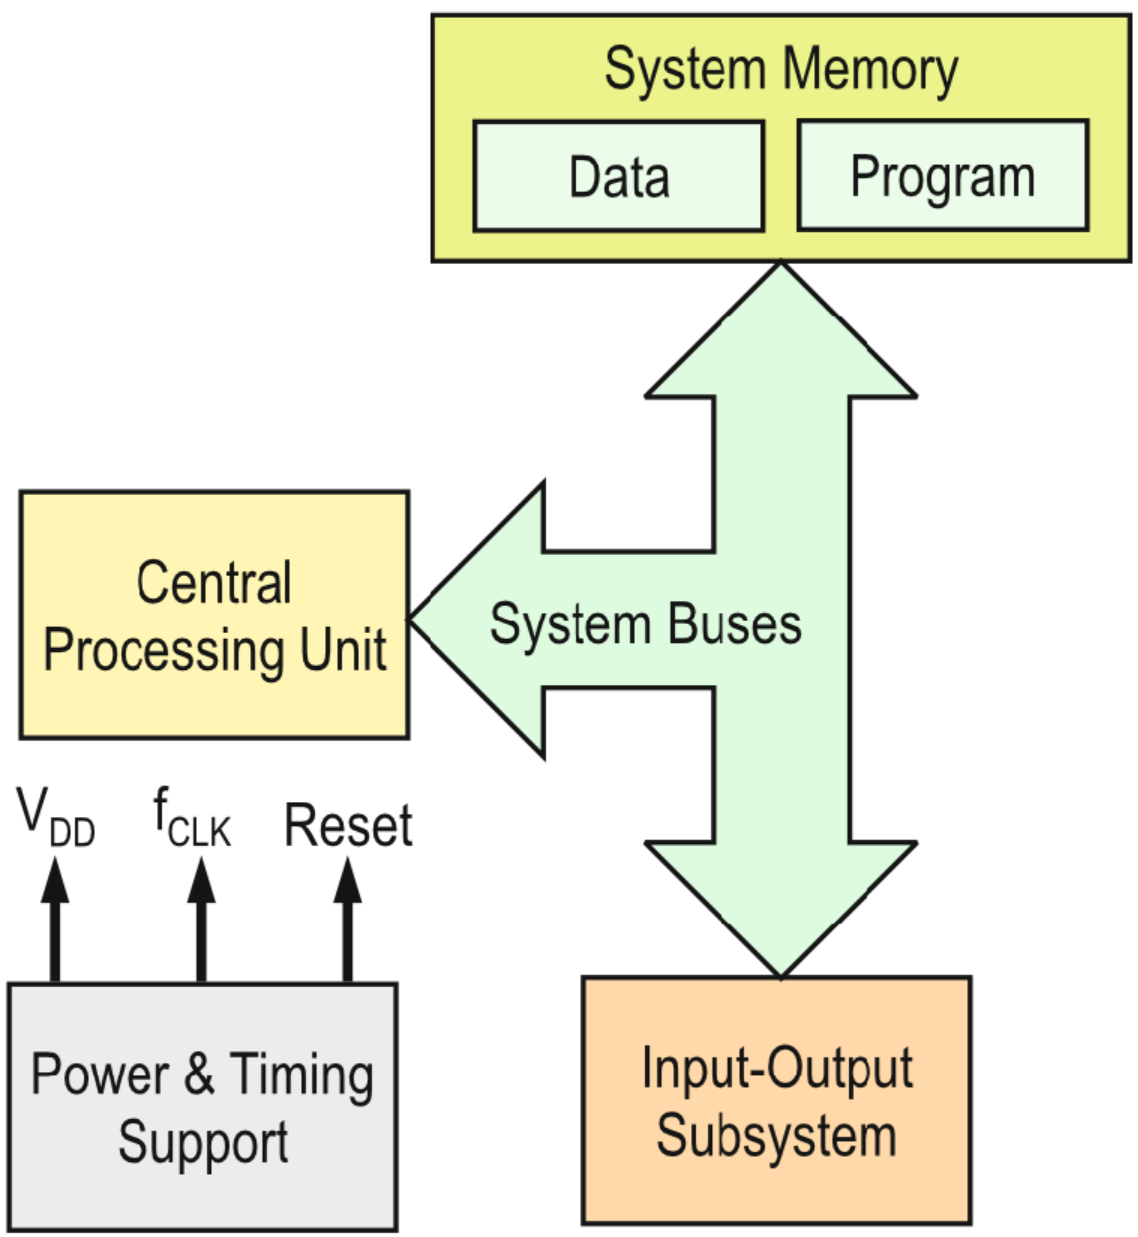
\includegraphics[width=0.8\linewidth]{images/uCArchitecture} 
\end{minipage}
\subsection{Microcontroller vs. Microprocessors}
\begin{multicols}{2}
		\subsubsection{Microprocessor(MPU)}
		\begin{itemize}
			\item Contain a General Purpose CPU
			\subitem ALU, CU, Registers, BIL %Bus Interface Logic
			\item Require External Components to form a Basic System
			\subitem Buses
			\subitem Memory
			\subitem I/O Interface \& Devices
			\item Additional Characteristics
			\subitem Architecture optimized for accelerating data processing
			\subitem Include elements to accelerate instruction execution  
		\end{itemize}
\subsubsection{Microcontroller(MCU)}
		\begin{itemize}
			\item Contain a Microprocessor Core
			\subitem Usually less complex than that of an MPU
			\item Include memory and peripherals in a single chip
			\subitem Denominated $ computer-on-a-chip $ 
			\subitem Most MCUs do not provide external buses
			\item On-chip Memory
			\subitem Includes both, Program and Data-memory
			\item Typical Peripherals
			\subitem Timers
			\subitem I/O ports
			\subitem Data converters
		\end{itemize}
\end{multicols}
\begin{center}
	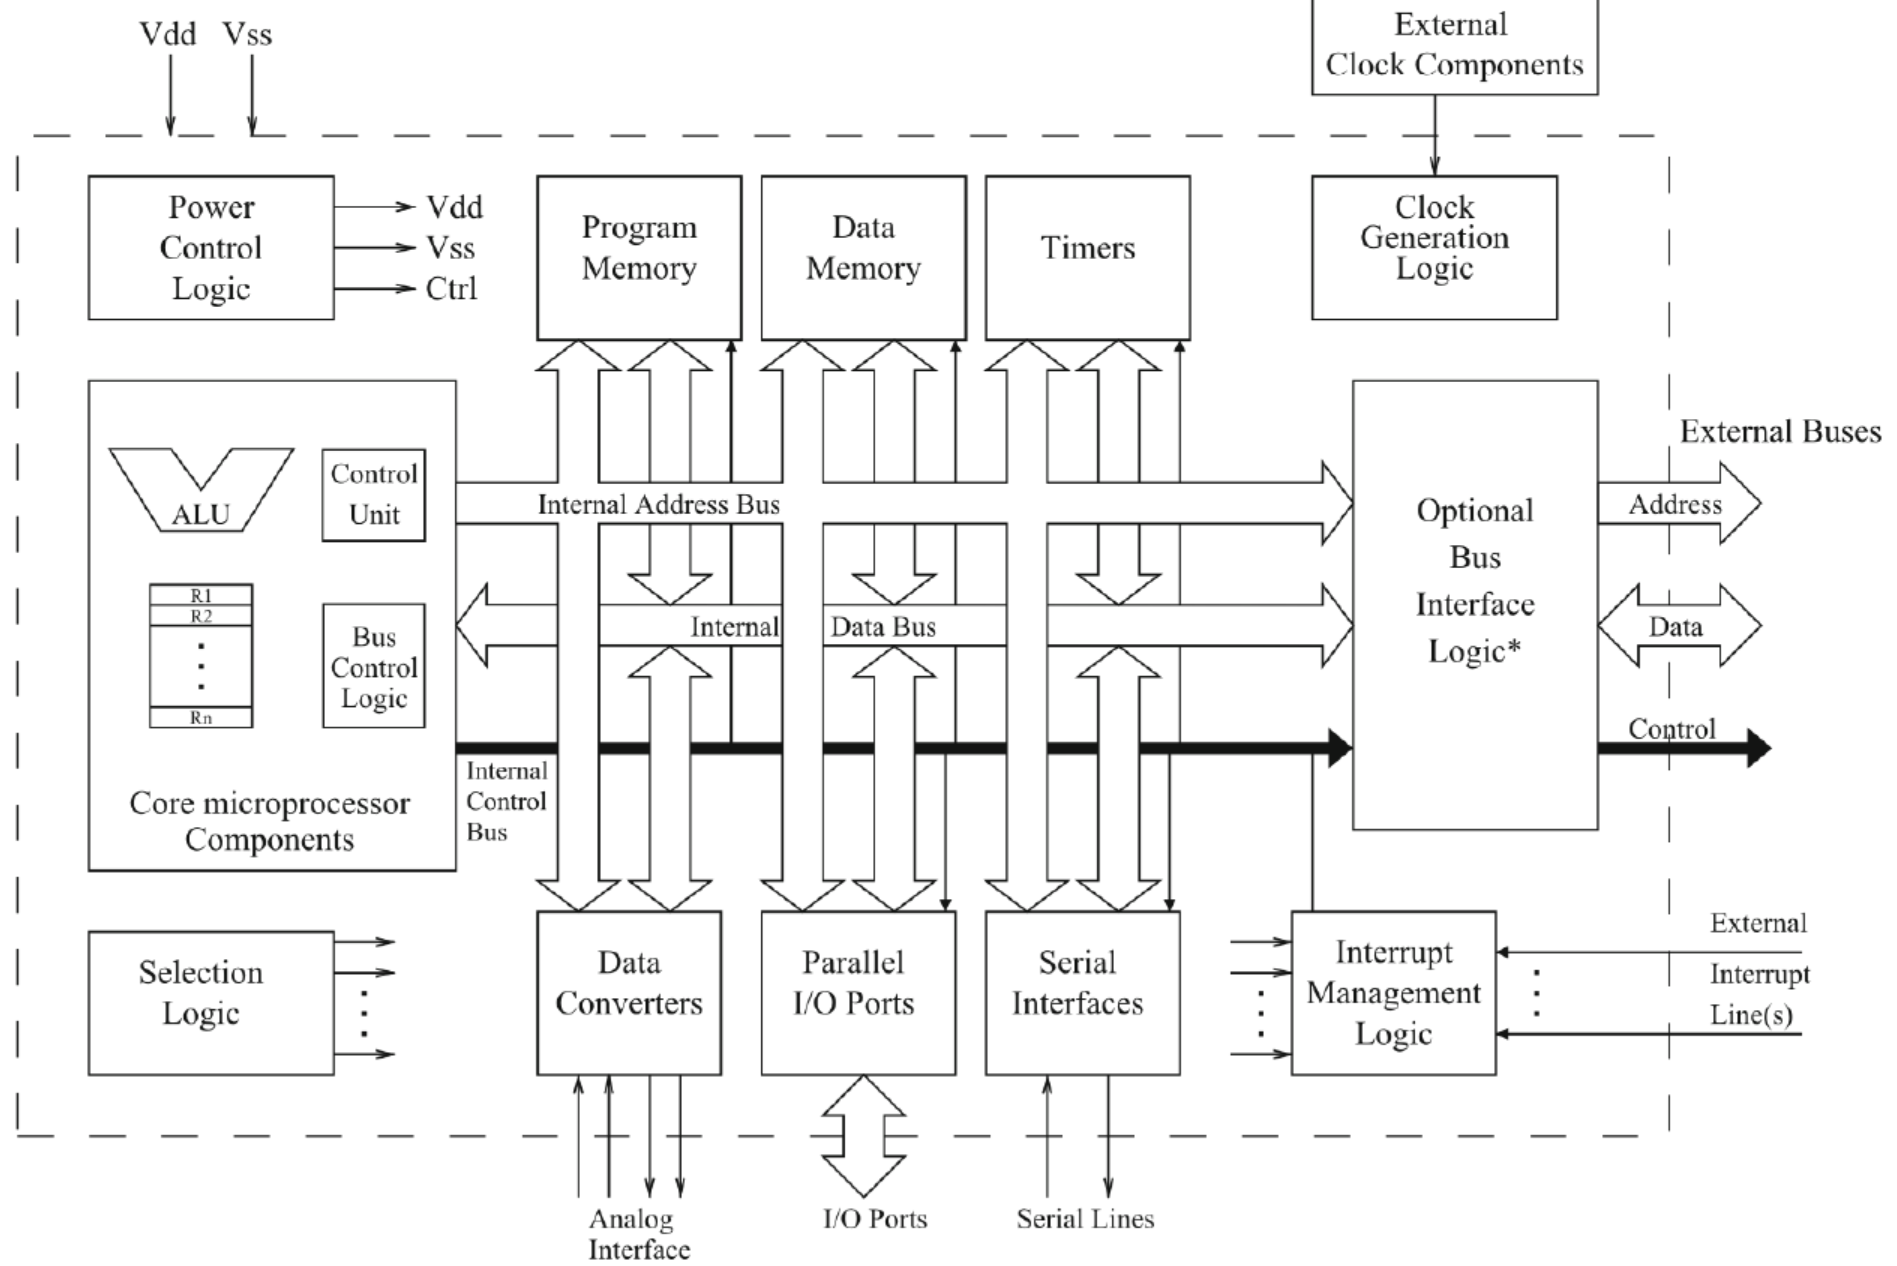
\includegraphics[width=9cm]{images/mCStructure}
\end{center}
\pagebreak

\subsection{RISC vs. CISC}
\begin{multicols}{2}
	\subsubsection{CISC (Complex Instruction Set Computer)}
		\begin{itemize}
			\item Variable length instructions
			\item Large instruction set
			\item Focuses in accomplishing as much as possible with each instruction
			\item Augments hardware complexity
			\item Simplifies programming
		\end{itemize}    
	\subsubsection{RISC (Reduced Instruction Set Computer)}
		\begin{itemize}
			\item Fixed length insructions
			\item Short instruction set
			\item Focuses on simple instructions
			\item Simplifies the hardware structure
			\item Makes programming harder
		\end{itemize}      
\end{multicols}

\begin{minipage}{8cm}
	\subsection{Central Processing Unit}
	\begin{itemize}
		\item Controll Unit (CU)
		\item Arithmetic Logic Unit (ALU)
		\item Register
		\item Bus Interface Logic (BIL)
	\end{itemize}
\end{minipage}
\begin{minipage}{6cm}
	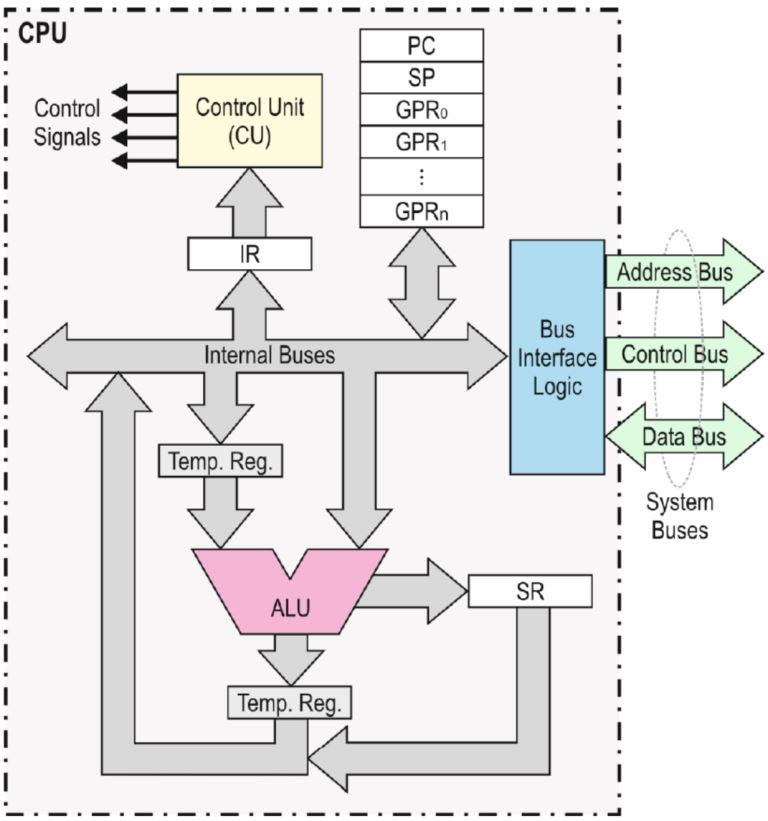
\includegraphics[width=6cm]{images/CPUComponents}
\end{minipage}

\begin{multicols}{2}
	\subsubsection{Control Unit (CU)}   
		\begin{itemize}
			\item Governs the CPU working
			\item Name of Cycles States: Fetch, Decode, Execute
			\item Also known als Infinite Loop or while(1)
		\end{itemize}
	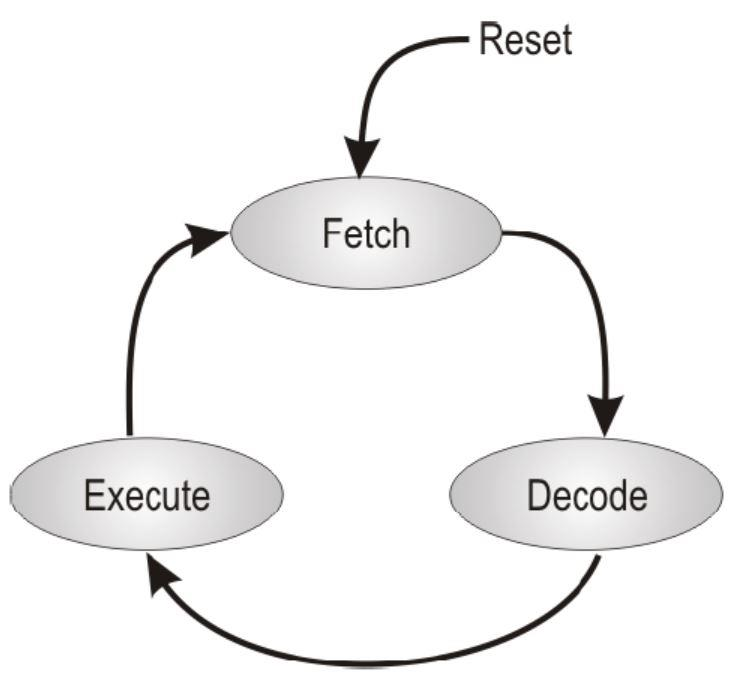
\includegraphics[width=4cm]{images/FDELoop}		
	\subsubsection{Arithmetic Logic Unit (ALU)}
	\begin{itemize}
		\item Performs Supported Logic and Arithmetic Operations
		\item 'Sets' the width of Databus and Registers
	\end{itemize}	
	\subsubsection{Bus Interface Logic (BIL)}
	\begin{itemize}
		\item Coordinates interaction between internal buses and system buses
		\item Define how adress, data and control buses works
	\end{itemize}	
	\subsubsection{Registers}
	\begin{itemize}
		\item Provide temporary storage in CPU
		\item Volatile Contents
		\item General and Special Purpose Registers
	\end{itemize}
	\subsubsection{General Purpose Regiser (GPR)}
	\begin{itemize}
		\item Not tied to specific functions
		\item Can hold data, variables, or addresses
		\item Number of registers depend on CPU architecture			
	\end{itemize}
	\subsubsection{Special Register (SR)}	
	\begin{itemize}
		\item Instruction Register (IR)
		\subitem Holds the current instruction 
		\item Programm Counter (PC)
		\subitem Holds the address of the next instruction to be fetched
		\item Stack Pointer (SP)
		\subitem Holds the address of the current top-of-stack 
		\item Status Register (SR)
		\subitem Holds the current CPU Status (Flags)
	\end{itemize}
\end{multicols}
\subsection{System Buses and Memory Organization}
\subsubsection{System Buses}
	\begin{itemize}
		\item Data Bus
		\subitem carrying data and instructions for read \&write
		\subitem bidirectional CPU $\leftrightarrow$ I/O or memory
		\item Adress bus
		\subitem Indicate Adress to be accessed
		\subitem number of memory which is adressable: 16Bit Bus $\rightarrow 2^{16}=64kB$ Memory
		\item Control bus
		\subitem regulate activity on buses		
	\end{itemize}
\subsubsection{Memory}
		\begin{itemize}
			\item The memory is organized as an array of cells
			\item Each memory location is identified by an adress
			\item The contents of a memory cell is a word
		\end{itemize}
	\begin{multicols}{2}
	\textbf{Memory Types}\\
	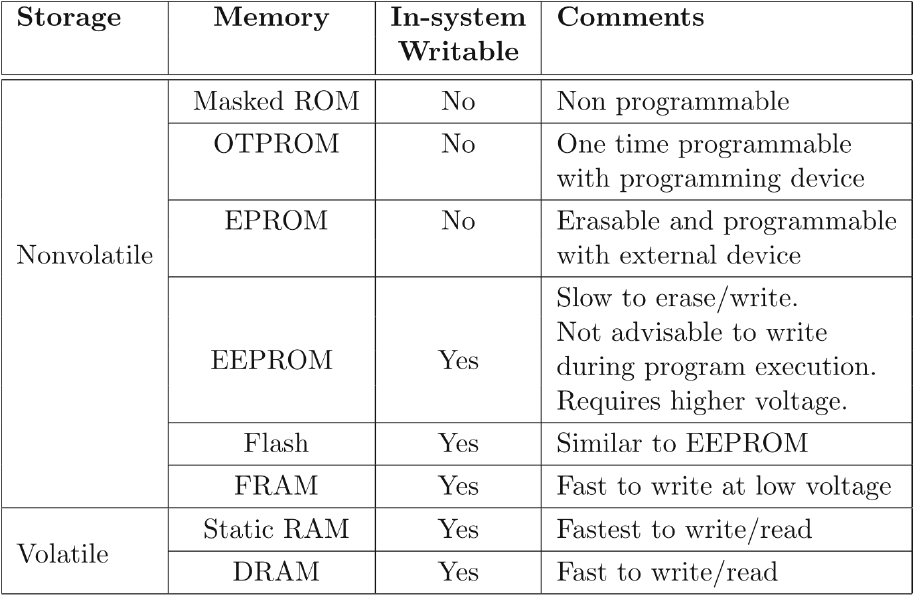
\includegraphics[width=8cm]{images/memorytypes.png}
	
	\textbf{Endianness}\\
	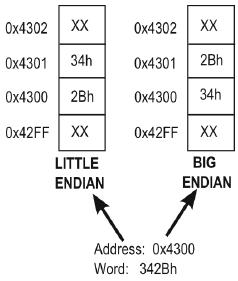
\includegraphics[width=5cm]{images/be_le.png}
	\end{multicols}
\subsubsection{Bus Architecture}
\begin{minipage}{9cm}
	\begin{itemize}
		\item Von Neumann
		\subitem A single bus for Instructions and Data
		\item Harvard
		\subitem Separate Bus for Instructions and Data
	\end{itemize}
\end{minipage}
\begin{minipage}{7cm}
	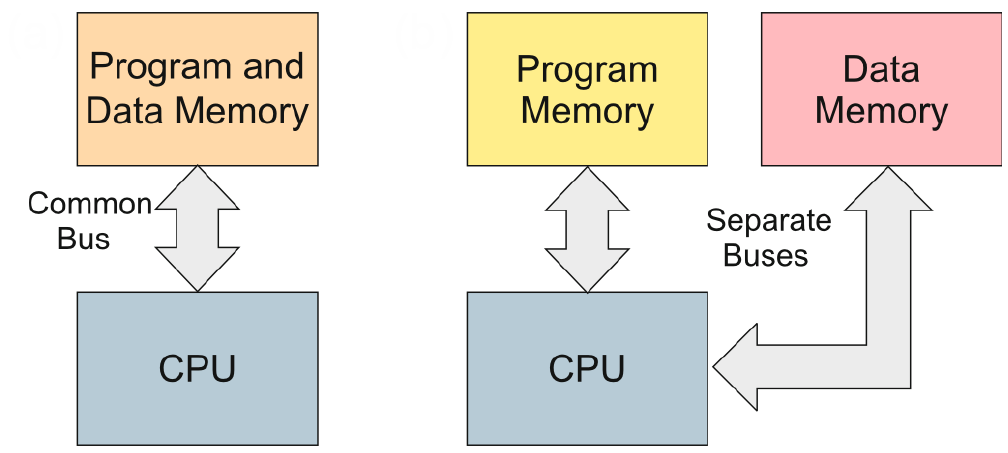
\includegraphics[width=7cm]{images/bus.png}
\end{minipage}

\subsection{I/O Subsystem}
Convers all the components other than the CPU \& memory connected to the system buses
\begin{itemize}
	\item Timers and Watchdog timers
	\item Communication interfaces
	\item Analog to Digital Converter (ADC)
	\item Digital to Analog Converter (DAC)
	\item Development peripherals
\end{itemize}
\begin{multicols}{2}
	\begin{minipage}{\linewidth}
		\textbf{Memory mapped I/O}\newline
		Address space inside the memory space, uses same instructions used to access memory
	\end{minipage}
	
	\begin{minipage}{\linewidth}
		\textbf{I/O mapped I/O} \newline
		Separate address space, instrutions, and signals for I/O (rarley used in modern processors)
	\end{minipage}
\end{multicols}
\begin{minipage}{0.6\linewidth}
	\textbf{IO Interface}\\
	\raggedright
	Include lines to connect to the system buses, I/O device connection lines and a set of internal registers
	\begin{tabular}{ll}
		\textbf{Control}  & to configure the operation of the device and interface  \\  
		\textbf{Status}   & to allow inquires about the device and interface status  \\ 
		\textbf{Data}     & for exchanging data with the device \\ 
	\end{tabular} 
\end{minipage}
\begin{minipage}{0.4\linewidth}
	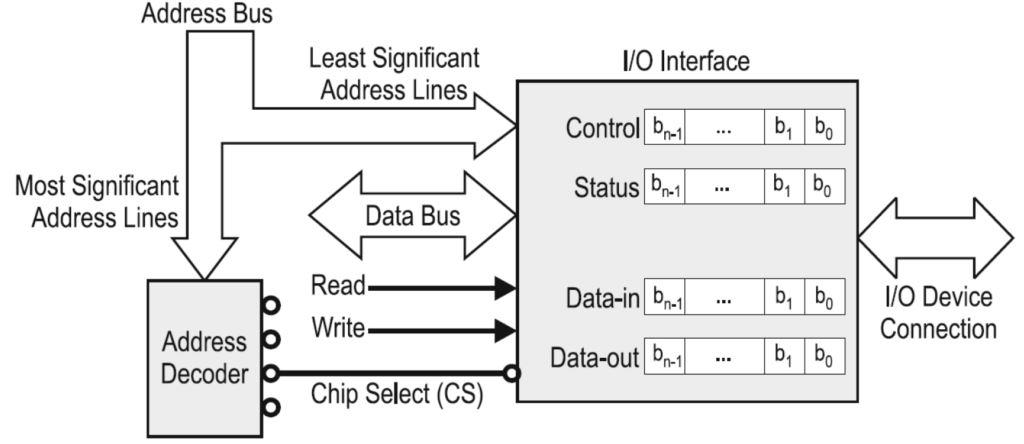
\includegraphics[width=\linewidth]{images/IOAnatomy} 
\end{minipage}

\clearpage
